

%%%%%%%%%%%%%%%%%%%%%%%%%%%%%%%%%%%%%%%%%%%%%%%%%%%%%%%
\subsubsection{Linear basis functions in tetrahedra ($P_1$)}
\index{general}{$P_1$}


\begin{verbatim}
(r_0,s_0) = (0,0,0)
(r_1,s_1) = (1,0,0)
(r_2,s_2) = (0,1,0)
(r_3,s_3) = (0,0,1)
\end{verbatim}

The basis polynomial is given by
\[
f(r,s,t)=c_0 + c_1 r + c_2 s + c_3 t
\]

\begin{eqnarray}
f_1 &=& f(r_1,s_1,t_1) = c_0 \\
f_2 &=& f(r_2,s_2,t_2) = c_0 + c_1\\
f_3 &=& f(r_3,s_3,t_3) = c_0 + c_2\\
f_4 &=& f(r_4,s_4,t_4) = c_0 + c_3
\end{eqnarray}

which yields:
\[
c_0=f_1
\quad
\quad
c_1=f_2-f_1
\quad
\quad
c_2=f_3-f_1
\quad
\quad
c_3=f_4-f_1
\]

\begin{eqnarray}
f(r,s,t) 
&=& c_0 + c_1 r + c_2 s + c_3 t \nonumber\\
&=& f_1 + (f_2-f_1) r + (f_3-f_1) s + (f_4-f_1) t \nonumber\\
&=& f_1 (1-r-s-t) + f_2 r + f_3 s + f_4 t \nonumber\\
&=& \sum_i N_i(r,s,t) f_i \nonumber
\end{eqnarray}

Finally,

\begin{mdframed}[backgroundcolor=blue!5]
\begin{eqnarray}
N_1(r,s,t) &=& 1-r-s-t \nonumber\\
N_2(r,s,t) &=& r \nonumber\\
N_3(r,s,t) &=& s \nonumber\\
N_4(r,s,t) &=& t \nonumber
\end{eqnarray}
\end{mdframed}

%%%%%%%%%%%%%%%%%%%%%%%%%%%%%%%%%%%%%%%%%%%%%%%%%%%%%%%
\subsubsection{Enriched linear in tetrahedra($P_1^+$)}
\index{general}{$P_1^+$}

These shape functions would be used in the MINI element, see Section~\ref{pair:mini}.

In 3D the buble function lools like $rst(1-r-s-t)$ so that 
\[
f(r,s,t)=a+b\; r+c\; s+d\; t+e \; rst(1-r-s-t)
\]
We have node 1 at location $(r,s,t)=(0,0,0)$, node 2 at $(r,s,t)=(1,0,0)$, node 3 at $(r,s,t)=(0,1,0)$ , 
node4 at $(r,s,t)=(0,0,1)$ and we 
set the location of the bubble (node 5) at $r=s=t=1/4$ so that 
\begin{eqnarray}
f(r_1,s_1,t_1)&=&f_1 = a+b\; r_1+c\; s_1+d\; t_1+e\; r_1s_1t_1(1-r_1-s_1-t_1) \\
f(r_2,s_2,t_2)&=&f_2 = a+b\; r_2+c\; s_2+d\; t_2+e\; r_2s_2t_2(1-r_2-s_2-t_2) \\
f(r_3,s_3,t_3)&=&f_3 = a+b\; r_3+c\; s_3+d\; t_3+e\; r_3s_3t_3(1-r_3-s_3-t_3) \\
f(r_4,s_4,t_4)&=&f_4 = a+b\; r_4+c\; s_4+d\; t_4+e\; r_4s_4t_4(1-r_4-s_4-t_4) \\ 
f(r_5,s_5,t_5)&=&f_5 = a+b\; r_5+c\; s_5+d\; t_5+e\; r_5s_5t_5(1-r_5-s_5-t_5) 
\end{eqnarray}
i.e.,
\begin{eqnarray}
f_1 &=& a\\
f_2 &=& a+b\\
f_3 &=& a+c\\
f_4 &=& a+d\\
f_5 &=& a+b/4+c/4+d/4+e/64 (1-1/4-1/4-1/4) \\ 
    &=& a+b/4+c/4+d/4+e/256  
\end{eqnarray}
Then 

\begin{eqnarray}
a&=&f_1\\
b&=&f_2-f_1\\
c&=&f_3-f_1\\
d&=&f_4-f_1\\
e&=&256(f_5-a-b/4-c/4-d/4) \\
&=&256(f_5-f_1-(f_2-f_1)/4-(f_3-f_1)/4-(f_4-f_1)/4) \\
&=&256(-f_1/4 - f_2/4 - f_3/4 - f_4/4 + f_5  ) \\
&=&64(-f_1 - f_2 - f_3 - f_4 + 4f_5  )
\end{eqnarray}
Finally:
\begin{eqnarray}
f(r,s,t)
&=& a+br+cs+dt+erst(1-r-s-t) \nn\\
&=& f_1 + (f_2-f_1)r + (f_3-f_1)s + (f_4-f_1)t+ 64(-f_1 - f_2 - f_3 - f_4 + 4f_5  ) rst(1-r-s-t)  \nn\\
&=& f_1 [1-r-s-t - 64rst(1-r-s-t)]\nn\\
&+& f_2 [r- 64rst(1-r-s-t)]\nn\\
&+& f_3 [s- 64rst(1-r-s-t)]\nn\\
&+& f_4 [t- 64rst(1-r-s-t)]\nn\\
&+& f_5 [256 rst(1-r-s-t)] \nn\\
&=&\sum_{i=1}^5 N_i(r,s,t) f_i
\end{eqnarray}
with
\begin{mdframed}[backgroundcolor=blue!5]
\begin{eqnarray}
N_1(r,s,t) &=& 1-r-s-t - 64rst(1-r-s-t) \\
N_2(r,s,t) &=& r - 64rst(1-r-s-t) \\
N_3(r,s,t) &=& s - 64rst(1-r-s-t) \\
N_4(r,s,t) &=& t - 64rst(1-r-s-t) \\
N_5(r,s,t) &=&  + 256rst(1-r-s-t) 
\end{eqnarray}
\end{mdframed}


%The question remains: in the papers about the MINI element, authors talk about adding the bubble function defined as
%$rs(1-r-s)$ in 2D but not about its coefficient. I am also curious about the isoparametric mapping. It seems to work, but would it be better/different with a simple P1 mapping?

The derivatives are given by:

\begin{eqnarray}
\frac{\partial N_1}{\partial r}(r,s,t) &=& -1 - 64st(1-2r-s-t) \nn\\
\frac{\partial N_2}{\partial r}(r,s,t) &=& +1 - 64st(1-2r-s-t) \nn\\
\frac{\partial N_3}{\partial r}(r,s,t) &=&    - 64st(1-2r-s-t) \nn\\
\frac{\partial N_4}{\partial r}(r,s,t) &=&    - 64st(1-2r-s-t) \nn\\
\frac{\partial N_5}{\partial r}(r,s,t) &=&     256st(1-2r-s-t) \nn\\ \nn\\ 
\frac{\partial N_1}{\partial s}(r,s,t) &=& -1 - 64rt(1-r-2s-t) \nn\\
\frac{\partial N_2}{\partial s}(r,s,t) &=&    - 64rt(1-r-2s-t) \nn\\
\frac{\partial N_3}{\partial s}(r,s,t) &=& +1 - 64rt(1-r-2s-t) \nn\\
\frac{\partial N_4}{\partial s}(r,s,t) &=&    - 64rt(1-r-2s-t) \nn\\
\frac{\partial N_5}{\partial s}(r,s,t) &=&     256rt(1-r-2s-t) \nn\\ \nn\\ 
\frac{\partial N_1}{\partial t}(r,s,t) &=& -1 - 64rs(1-r-s-2t) \nn\\
\frac{\partial N_2}{\partial t}(r,s,t) &=&    - 64rs(1-r-s-2t) \nn\\
\frac{\partial N_3}{\partial t}(r,s,t) &=&    - 64rs(1-r-s-2t) \nn\\
\frac{\partial N_4}{\partial t}(r,s,t) &=& +1 - 64rs(1-r-s-2t) \nn\\
\frac{\partial N_5}{\partial t}(r,s,t) &=&     256rs(1-r-s-2t) \nn
\end{eqnarray}






%%%%%%%%%%%%%%%%%%%%%%%%%%%%%%%%%%%%%%%%%%%%%%%%%%%%%%%
\subsubsection{Triquadratic basis functions in 3D ($Q_2$)}
\index{general}{$Q_2$}

\begin{verbatim}
   t
   |
   .--s
  /
 r
                                    05=====16=====08 
                                    |      |      |  
                                    |      |      |  
                  13=====26=====15  17=====25=====20 
                  |      |      |   |      |      |  
                  |      |      |   |      |      |  
06=====14=====07  22=====27=====24  01=====12=====04 @ r=-1
|      |      |   |      |      |  
|      |      |   |      |      |   
18=====23=====14  09=====21=====11 @ r=0
|      |      |   
|      |      |  
02=====10=====03 @ r=+1
\end{verbatim}





\begin{eqnarray}
N_{1}&=& 0.5r(r-1)  \;0.5s(s-1)\; 0.5t(t-1)  \nonumber\\
N_{2}&=& 0.5r(r+1)  \;0.5s(s-1)\; 0.5t(t-1)  \nonumber\\
N_{3}&=& 0.5r(r+1)  \;0.5s(s+1)\; 0.5t(t-1)  \nonumber\\
N_{4}&=& 0.5r(r-1)  \;0.5s(s+1)\; 0.5t(t-1)  \nonumber\\
N_{5}&=& 0.5r(r-1)  \;0.5s(s-1)\; 0.5t(t+1)  \nonumber\\
N_{6}&=& 0.5r(r+1)  \;0.5s(s-1)\; 0.5t(t+1)  \nonumber\\
N_{7}&=& 0.5r(r+1)  \;0.5s(s+1)\; 0.5t(t+1)  \nonumber\\
N_{8}&=& 0.5r(r-1)  \;0.5s(s+1)\; 0.5t(t+1)  \nonumber\\
N_{9}&=& (1-r^2)   \;0.5s(s-1)\; 0.5t(t-1)  \nonumber\\
N_{10}&=& 0.5r(r+1) \;(1-s^2)  \; 0.5t(t-1)  \nonumber\\
N_{11}&=& (1-r^2)  \;0.5s(s+1)\; 0.5t(t-1)  \nonumber\\
N_{12}&=& 0.5r(r-1) \;(1-s^2)  \; 0.5t(t-1)  \nonumber\\
N_{13}&=& (1-r^2)  \;0.5s(s-1)\; 0.5t(t+1)  \nonumber\\
N_{14}&=& 0.5r(r+1) \;(1-s^2)  \; 0.5t(t+1)  \nonumber\\
N_{15}&=& (1-r^2)  \;0.5s(s+1)\; 0.5t(t+1)  \nonumber\\
N_{16}&=& 0.5r(r-1) \;(1-s^2)  \; 0.5t(t+1)  \nonumber\\
N_{17}&=& 0.5r(r-1) \;0.5s(s-1)\; (1-t^2)  \nonumber\\
N_{18}&=& 0.5r(r+1) \;0.5s(s-1)\; (1-t^2)  \nonumber\\
N_{19}&=& 0.5r(r+1) \;0.5s(s+1)\; (1-t^2)  \nonumber\\
N_{20}&=& 0.5r(r-1) \;0.5s(s+1)\; (1-t^2)  \nonumber\\
N_{21}&=& (1-r^2)   \;(1-s^2)  \; 0.5t(t-1)  \nonumber\\
N_{22}&=& (1-r^2)   \;0.5s(s-1)\; (1-t^2)  \nonumber\\
N_{23}&=& 0.5r(r+1) \;(1-s^2)  \; (1-t^2)  \nonumber\\
N_{24}&=& (1-r^2)   \;0.5s(s+1)\; (1-t^2)  \nonumber\\
N_{25}&=& 0.5r(r-1) \;(1-s^2)  \; (1-t^2)  \nonumber\\
N_{26}&=& (1-r^2)   \;(1-s^2)  \; 0.5t(t+1)  \nonumber\\
N_{27}&=& (1-r^2)   \;(1-s^2)  \; (1-t^2)  \nonumber
\end{eqnarray}

%.....................................................................
\subsubsection{Enriched quadratic basis functions in tetrahedra ($P_2^+$)}
\index{general}{$P_2^+$}

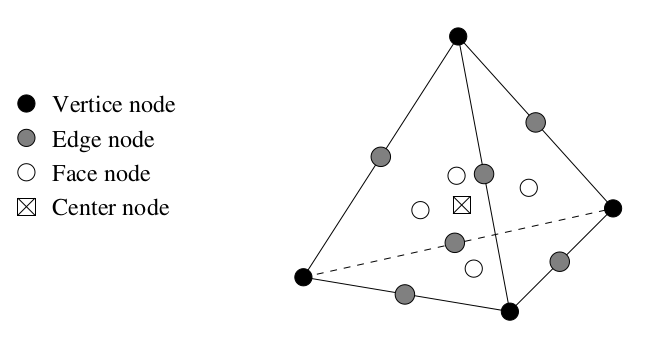
\includegraphics[width=9cm]{images/crouzeix-raviart/p2pp1_3D1}
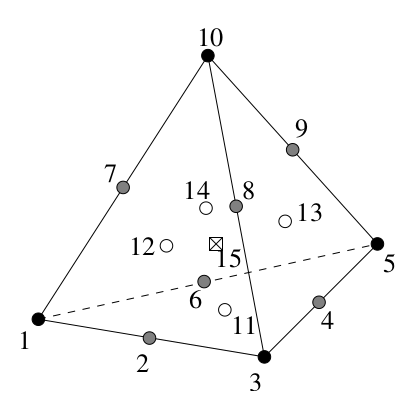
\includegraphics[width=5cm]{images/crouzeix-raviart/p2pp1_3D2}

The velocity shape functions are:
\begin{eqnarray}
\phi_i &=& \lambda_i(2\lambda_i-1) + 3 (\lambda_i\lambda_j \lambda_k + \lambda_i\lambda_j\lambda_l + \lambda_i\lambda_k\lambda_l) -4 \lambda_i\lambda_j\lambda_k\lambda_l \\
\phi_{ij} &=& 4\lambda_i\lambda_j - 12( \lambda_i\lambda_j\lambda_k+\lambda_i\lambda_j\lambda_l  ) +32 \lambda_i\lambda_j\lambda_k \lambda_l \\
\phi_{ijk} &=& 27  \lambda_i\lambda_j\lambda_k - 108 \lambda_i\lambda_j\lambda_k \lambda_l \\
\phi_c &=& 256 \lambda_i\lambda_j\lambda_k\lambda_l
\end{eqnarray}

\todo[inline]{REFS ??? better definition of functions !}

%.....................................................................
\subsubsection{Linear basis functions for hexahedra ($P_1$)} \label{ss:lbfh3D}
\index{general}{$P_1$}

This is essentially in the $Q_2\times P_{-1}$ element. 
I choose the reduced coordinates of the pressure nodes to be :

\begin{tabular}{cccc}
\hline
point & r & s & t \\
\hline
1& 1/2 &-1/2 &-1/2\\
2& -1/2 &1/2 &-1/2\\
3& -1/2 &-1/2& 1/2\\
4& 1/2 &1/2& 1/2 \\
\hline
\end{tabular}

Inside the element the pressure is given as a linear function of the reduced coordinates $r,s,t$:
\[
p(r,s,t)=a+br+cs+dt
\]
This expression must exactly interpolate the pressure at all four pressure nodes:
\begin{eqnarray}
p_1 
&=& p(r_1,s_1,t_1) 
= a+br_1+cs_1+dt_1 
= a+b/2-c/2-d/2\nonumber\\
p_2
&=& p(r_2,s_2,t_2)
= a+br_2+cs_2+dt_2
= a-b/2+c/2-d/2\nonumber\\
p_3
&=& p(r_3,s_3,t_3) 
= a+br_3+cs_3+dt_3 
= a-b/2-c/2+d/2\nonumber\\
p_4
&=& p(r_4,s_4,t_4) 
= a+br_4+cs_4+dt_4
= a+b/2+c/2+d/2\nonumber
\end{eqnarray}
or,
\begin{equation}
\left(
\begin{array}{cccc}
1 & 1/2 & -1/2 & -1/2 \\
1 & -1/2 & +1/2 & -1/2 \\
1 & -1/2 & -1/2 & +1/2 \\
1 & 1/2 & +1/2 & +1/2 
\end{array}
\right)
\left(
\begin{array}{c}
a\\b\\c\\d
\end{array}
\right)=
\left(
\begin{array}{c}
p_1\\p_2\\p_3\\p_4
\end{array}
\right)
\nonumber
\end{equation}

The matrix is invertible and we get:
\[
\left(
\begin{array}{c}
a\\b\\c\\d
\end{array}
\right)=
\left(
\begin{array}{cccc}
1/4 & 1/4 & 1/4 & 1/4 \\
1/2 & -1/2 & -1/2 & 1/2 \\
-1/2 & 1/2 & -1/2 & 1/2 \\
-1/2 & -1/2 & 1/2 & 1/2
\end{array}
\right)
\left(
\begin{array}{c}
p_1\\p_2\\p_3\\p_4
\end{array}
\right)
\]

so 
\begin{eqnarray}
p(r,s,t)
&=& a+br+cs+dt \nonumber\\
&=& \frac{1}{4}(p_1+p_2+p_3+p_4)
+\frac{1}{2}(p_1-p_2-p_3+p_4)r
+\frac{1}{2}(-p_1+p_2-p_3+p_4)s
+\frac{1}{2}(-p_1-p_2+p_3+p_4)t\nonumber\\
&=&
\frac{1}{4}(1+2r-2s-2t)p_1+
\frac{1}{4}(1-2r+2s-2t)p_2+
\frac{1}{4}(1-2r-2s+2t)p_3+
\frac{1}{4}(1+2r+2s+2t)p_4 \nonumber\\
&=& \sum_{i=1}^4 N_i(r,s,t) p_i
\end{eqnarray}
with
\begin{eqnarray}
N_1(r,s,t) &=& \frac{1}{4}(1+2r-2s-2t)\nonumber\\
N_2(r,s,t) &=& \frac{1}{4}(1-2r+2s-2t)\nonumber\\
N_3(r,s,t) &=& \frac{1}{4}(1-2r-2s+2t)\nonumber\\
N_4(r,s,t) &=& \frac{1}{4}(1+2r+2s+2t)\nonumber
\end{eqnarray}

\vspace{.6cm}

I could also have chosen 

\begin{tabular}{cccc}
\hline
point & r & s & t \\
\hline
1& 0 & 0 &0 \\
2& 1 & 0 &0 \\
3& 0 & 1 &0 \\
4& 0 & 0 &1 \\
\hline
\end{tabular}

This expression must exactly interpolate the pressure at all four pressure nodes:
\begin{eqnarray}
p_1  &=& p(r_1,s_1,t_1) = a+br_1+cs_1+dt_1 = a\nonumber\\
p_2  &=& p(r_2,s_2,t_2) = a+br_2+cs_2+dt_2 = a+b\nonumber\\
p_3  &=& p(r_3,s_3,t_3) = a+br_3+cs_3+dt_3 = a+c\nonumber\\
p_4  &=& p(r_4,s_4,t_4) = a+br_4+cs_4+dt_4 = a+d\nonumber
\end{eqnarray}
i.e.
\[
a=p_1
\qquad
b=p_2-p1
\qquad
c=p_3-p1
\qquad
d=p_4-p1
\]
or, 
\[
p^h(r,s)=a+br+cs+dt=p_1 + (p_2-p_1)r + (p_3-p_1)r + (p_4-p_1)t  = p_1(1-r-s-t) + r p_2 + s p_3 + t p_4
\]
so 
\begin{mdframed}[backgroundcolor=blue!5]
\begin{eqnarray}
N_1(r,s,t) &=& 1-r-s-t \\ 
N_2(r,s,t) &=& r \\
N_3(r,s,t) &=& s \\
N_4(r,s,t) &=& t
\end{eqnarray}
\end{mdframed}






%%%%%%%%%%%%%%%%%%%%%%%%%%%%%%%%%%%%%%%%%%%%%%%%%%%%%%%%%%%%%%%%%%%%%
\subsubsection{20-node serendipity basis functions in 3D ($Q_2^{(20)}$)}
\index{general}{$Q_2^{(20)}$} \index{general}{Serendipity element}

The serendipity elements are those rectangular elements which have no
interior nodes \cite[p91]{reddybook2}.

\begin{verbatim}
   t
   |
   .--s
  /
 r
                                    05=====20=====08 
                                    |             |  
                                    |             |  
                  17 - - - - - -19  13            16
                  .              .  |             |  
                  .              .  |             |  
06=====18=====07  .              .  01=====12=====04 @ r=-1
|             |   .              . 
|             |   .              .  
14            15  09 - - - - - -11 @ r=0
|             |   
|             |  
02=====10=====03 @ r=+1
\end{verbatim}

\todo[inline]{find/build shape functions!}


%..........................................................................---------------------------
\subsubsection{Enriched linear basis functions in quadrilaterals ($Q_1^+$) -WIP} \label{ss:quadmini3D}
\index{general}{$Q_1^+$}

Following Lamichhane (2017) \cite{lami17} we can define two bubble functions to enrich the 
$Q_1$ space:

\begin{eqnarray}
b^{(1)} (r,s,t) &=& (1-r)(1-s)(1-t) \cdot (1-r^2) (1-s^2) (1-t^2) \\
b^{(2)} (r,s,t) &=& (1 + \beta(r+s+t)) \cdot (1-r^2) (1-s^2) (1-t^2) 
\end{eqnarray}

The first one includes a tri-linear term while the second one includes a linear one parameterised by $\beta$.
In both cases the bubble is identically zero on the edges of the reference element and it is exactly 1 
in its middle.

\begin{eqnarray}
\frac{\partial b^{(1)}}{\partial r}(r,s,t) &=& (3r^2-2r-1)(1-s)(1-s^2)(1-t)(1-t^2) \\ 
\frac{\partial b^{(1)}}{\partial s}(r,s,t) &=& (3s^2-2s-1)(1-r)(1-r^2)(1-t)(1-t^2) \\ 
\frac{\partial b^{(1)}}{\partial t}(r,s,t) &=& (3t^2-2t-1)(1-r)(1-r^2)(1-s)(1-s^2)  
\end{eqnarray}

\begin{eqnarray}
\frac{\partial b^{(2)}}{\partial r}(r,s,t) &=&  -[b(3r^2+2r(s+t)-1)+2r](1-s^2)(1-t^2)\\
\frac{\partial b^{(2)}}{\partial s}(r,s,t) &=&  -[b(3s^2+2s(r+t)-1)+2s](1-r^2)(1-t^2)\\
\frac{\partial b^{(2)}}{\partial t}(r,s,t) &=&  -[b(3t^2+2t(r+s)-1)+2t](1-r^2)(1-s^2)
\end{eqnarray}





%-----------------------------------------------------------------
\subsubsection{The rotated $Q_1$} \label{ss:rq1}
\index{general}{$\tilde{Q}_1$}

The nodes are not on the corners of the element but in the middle of the
element faces:

\begin{center}
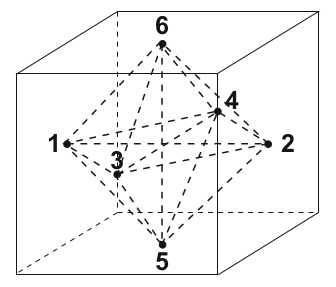
\includegraphics[width=4cm]{images/rannacherturek/elt3D}\\
{\captionfont Node numbering and connectivity pattern of the reference element. Taken from \cite{gekm08}}
\end{center}

We have $\tilde{Q}_1=span \{1,r,s,t,r^2-s^2,s^2-t^2\}$.

%.............................................
\paragraph{The Middle Point (MP) variant}. 

The shape functions are given by (see Georgiev et al (2008) \cite{gekm08}):
\begin{eqnarray}
N_1(r,s,t) &=& \frac{1}{6}(1-3r+2r^2-s^2-t^2 ) \\
N_2(r,s,t) &=& \frac{1}{6}(1+3r+2r^2-s^2-t^2 ) \\
N_3(r,s,t) &=& \frac{1}{6}(1-r^2-3s+2s^2-t^2 ) \\
N_4(r,s,t) &=& \frac{1}{6}(1-r^2+3s+2s^2-t^2 ) \\
N_5(r,s,t) &=& \frac{1}{6}(1-r^2-s^2-3t+2t^2 ) \\
N_6(r,s,t) &=& \frac{1}{6}(1-r^2-s^2+3t+2t^2 ) 
\end{eqnarray}

\begin{eqnarray}
\frac{\partial N_1}{\partial r} &=& \frac{1}{6} (-3+4r )\\
\frac{\partial N_2}{\partial r} &=& \frac{1}{6} (3+4r )\\
\frac{\partial N_3}{\partial r} &=& \frac{1}{6} (-2r) \\
\frac{\partial N_4}{\partial r} &=& \frac{1}{6} (-2r) \\
\frac{\partial N_5}{\partial r} &=& \frac{1}{6} (-2r) \\
\frac{\partial N_6}{\partial r} &=& \frac{1}{6} (-2r) 
\end{eqnarray}

\begin{eqnarray}
\frac{\partial N_1}{\partial s} &=& \frac{1}{6} (-2s)\\ 
\frac{\partial N_2}{\partial s} &=& \frac{1}{6} (-2s) \\
\frac{\partial N_3}{\partial s} &=& \frac{1}{6} (-3+4s )\\
\frac{\partial N_4}{\partial s} &=& \frac{1}{6} (3+4s )\\
\frac{\partial N_5}{\partial s} &=& \frac{1}{6} (-2s) \\
\frac{\partial N_6}{\partial s} &=& \frac{1}{6} (-2s) 
\end{eqnarray}

\begin{eqnarray}
\frac{\partial N_1}{\partial t} &=& \frac{1}{6}(-2t) \\ 
\frac{\partial N_2}{\partial t} &=& \frac{1}{6}(-2t) \\ 
\frac{\partial N_3}{\partial t} &=& \frac{1}{6}(-2t) \\ 
\frac{\partial N_4}{\partial t} &=& \frac{1}{6}(-2t) \\ 
\frac{\partial N_5}{\partial t} &=& \frac{1}{6}(-3+4t) \\ 
\frac{\partial N_6}{\partial t} &=& \frac{1}{6}(3+4t)  
\end{eqnarray}


%......................................
\paragraph{The Mid Value (MV) variant}. 

\begin{eqnarray}
N_1(r,s,t) &=& \frac{1}{12}(2-6r+6r^2-3s^2-3t^2) \\
N_2(r,s,t) &=& \frac{1}{12}(2+6r+6r^2-3s^2-3t^2) \\
N_3(r,s,t) &=& \frac{1}{12}(2-3r^2-6s+6s^2-3t^2) \\
N_4(r,s,t) &=& \frac{1}{12}(2-3r^2+6s+6s^2-3t^2) \\
N_5(r,s,t) &=& \frac{1}{12}(2-3r^2-3s^2-6t+6t^2) \\
N_6(r,s,t) &=& \frac{1}{12}(2-3r^2-3s^2+6t+6t^2)
\end{eqnarray}

\begin{eqnarray}
\frac{\partial N_1}{\partial r} &=& \frac{1}{12}(-6+12r) = \frac{1}{2}(-1+2r)\\
\frac{\partial N_2}{\partial r} &=& \frac{1}{12}(6+12r) = \frac{1}{2}(1+2r)\\
\frac{\partial N_3}{\partial r} &=& \frac{1}{12}(-6r) = -\frac{1}{2}r \\
\frac{\partial N_4}{\partial r} &=& \frac{1}{12}(-6r) = -\frac{1}{2}r \\
\frac{\partial N_5}{\partial r} &=& \frac{1}{12}(-6r) = -\frac{1}{2}r \\
\frac{\partial N_6}{\partial r} &=& \frac{1}{12}(-6r) = -\frac{1}{2}r 
\end{eqnarray}

\begin{eqnarray}
\frac{\partial N_1}{\partial s} &=& \frac{1}{12} (-6s) = -\frac{1}{2}s \\
\frac{\partial N_2}{\partial s} &=& \frac{1}{12} (-6s) = -\frac{1}{2}s \\
\frac{\partial N_3}{\partial s} &=& \frac{1}{12} (-6+12s) = \frac{1}{2} (-1+2s) \\ 
\frac{\partial N_4}{\partial s} &=& \frac{1}{12} (6+12s) = \frac{1}{2} (1+2s) \\ 
\frac{\partial N_5}{\partial s} &=& \frac{1}{12} (-6s) = -\frac{1}{2}s \\
\frac{\partial N_6}{\partial s} &=& \frac{1}{12} (-6s) = -\frac{1}{2}s 
\end{eqnarray}

\begin{eqnarray}
\frac{\partial N_1}{\partial t} &=& \frac{1}{12} (-6t) = -\frac{1}{2}t \\
\frac{\partial N_2}{\partial t} &=& \frac{1}{12} (-6t) = -\frac{1}{2}t \\
\frac{\partial N_3}{\partial t} &=& \frac{1}{12} (-6t) = -\frac{1}{2}t \\
\frac{\partial N_4}{\partial t} &=& \frac{1}{12} (-6t) = -\frac{1}{2}t \\
\frac{\partial N_5}{\partial t} &=& \frac{1}{12} (-6+12t) = \frac{1}{2} (-1+2t) \\ 
\frac{\partial N_6}{\partial t} &=& \frac{1}{12} (6+12t) = \frac{1}{2} (1+2t) 
\end{eqnarray}






%-----------------------------------------------------------------
\subsubsection{The 3D enriched $Q_1^+\times P_0$ of Fortin} \label{ss:Q1pP0}

This element is mentioned on p249 of Cuvelier, Segal \& van Steenhoven \cite{cuss86}:
"The enriched trilinear velocity-constant pressure element is probably the simplest admissible 3D element."
Fortin \cite{fort81} designed a simple LBB-stable $Q_1$ element to which mid-face nodes are added, 
i.e. a 'bubble' $Q_2$ function is added on each face.
However, only $\vec\upnu\cdot \vec{n}$ is present on these mid-face nodes: 

\begin{flushright} {\tiny {\color{gray} (tikz\_q1pp0.tex)}} \end{flushright}
%~~~~~~~~~~~~~~~~~~~~~~~~~~~~~~~~~~~~~~~~~~~~~~~~~~~~~~~~~~~~~~~~~~~~~~~~~~~~~~~~~~~~~~~~~~~~~~~~~~

\begin{center}
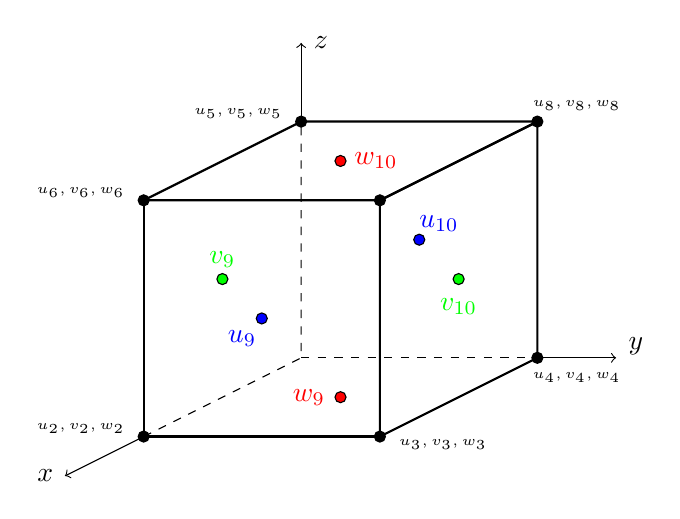
\begin{tikzpicture}
%\draw[fill=gray!23,gray!23](0,0) rectangle (9,7);
%\draw[step=0.5cm,gray,very thin] (0,0) grid (9,7); %background grid

\draw[thick] (2,4.5) -- (5,4.5) -- (7,5.5) -- (4,5.5) -- cycle; %top
\draw[thick] (2,1.5) -- (5,1.5) -- (5,4.5) -- (2,4.5) -- cycle; %front
\draw[thick] (5,1.5) -- (7,2.5) -- (7,5.5) -- (5,4.5) -- cycle; %right

\draw[dashed]   (2,1.5) -- (4,2.5) -- (4,5.5) ; % 
\draw[dashed]   (4,2.5) -- (7,2.5)  ; % 

\draw[thin,->] (2,1.5) -- (1,1); %x
\draw[thin,->] (7,2.5) -- (8,2.5); %y
\draw[thin,->] (4,5.5) -- (4,6.5); %z
\node[] at (0.75,1) {$x$};
\node[] at (8.25,2.65) {$y$};
\node[] at (4.25,6.5) {$z$};

\draw[black,fill=black] (2,1.5)   circle (2pt);
\draw[black,fill=black] (5,1.5)   circle (2pt);
\draw[black,fill=black] (5,4.5)   circle (2pt);
\draw[black,fill=black] (2,4.5)   circle (2pt);
\draw[black,fill=black] (7,2.5)  circle (2pt);
\draw[black,fill=black] (7,5.5)  circle (2pt);
\draw[black,fill=black] (4,5.5) circle (2pt);

\node[] at (1.2,1.6) {\tiny $u_2,v_2,w_2$};
\node[] at (5.8,1.4) {\tiny $u_3,v_3,w_3$};
\node[] at (7.5,2.25) {\tiny $u_4,v_4,w_4$};
\node[] at (3.2,5.6) {\tiny $u_5,v_5,w_5$};
\node[] at (1.2,4.6) {\tiny $u_6,v_6,w_6$};
\node[] at (7.5,5.7) {\tiny $u_8,v_8,w_8$};

\draw[black,fill=blue] (3.5,3) circle (2pt); 
\draw[black,fill=blue] (5.5,4) circle (2pt); 
\node[] at (3.25,2.75) {\color{blue} $u_9$};
\node[] at (5.75,4.2) {\color{blue} $u_{10}$};

\draw[black,fill=green] (3,3.5) circle (2pt); 
\draw[black,fill=green] (6,3.5) circle (2pt); 
\node[] at (3,3.75) {\color{green} $v_9$};
\node[] at (6,3.15) {\color{green} $v_{10}$};

\draw[black,fill=red] (4.5,2) circle (2pt); 
\draw[black,fill=red] (4.5,5) circle (2pt); 
\node[] at (4.1,2) {\color{red} $w_9$};
\node[] at (4.95,5) {\color{red} $w_{10}$};

\end{tikzpicture}\\
\end{center}



Fortin states: "this element satisfies the B.B. condition and is probably the simplest 3-D element to do SO. This
unfortunately does not mean that it is more accurate (at least on regular meshes)." and 
"the element satisfies the B.B. condition. It can therefore be used in a non-regular mesh without fear. The number of
degrees of freedom is approximately double with respect to the $Q_1\times P_0$ element and this is
reflected by an increased number of vortices and a reduction of their size. However, there
seems to be a qualitative deficiency of these vortices since they do not easily assemble into
complex flows. Only numerical experiments can give the final answer."

Considering a single element, we have 
\begin{itemize}
\item $Q_1$: $2\times 2\times 2\times 3=24$ velocity dofs
\item $Q_1^+$: $2\times 2\times 2\times 3+6 = 30$ velocity dofs: 
\[
\vec{V}^T=(\underbrace{u_1,v_1,w_1,\dots,u_8,v_8,w_8}_{Q_1\; dofs},
\underbrace{u_9,v_9,w_9,u_{10},v_{10},w_{10}}_{bubble \; dofs})
\]
The big difference with all other elements so far is the fact that the dofs $u_9,v_9,w_9$ are not colocated (same
for the other three). $u_9$ lives in the middle of the $r=-1$ face, $v_9$ lives in the middle of the $s=-1$ face and 
$w_9$ lives in the middle of the $t=-1$ face.


\item $Q_2$: $3\times 3\times 3\times 3=81$ velocity dofs 
\end{itemize}

Considering a 3D mesh composed of $nel=nelx\times nely\times nelz$ elements:
\begin{itemize}
\item $Q_1$: the total number of Velocity dofs is $NfemV=(nelx+1)\times(nely+1)\times(nelz+1)\times 3$
\item $Q_1^+$:  the total number of nodes is 
\[NfemV=(nelx+1)\times(nely+1)\times(nelz+1)\times 3 
+ (nelx+1)\times nely\times nelz
+ nelx\times (nely+1)\times nelz
+ nelx\times nely \times (nelz+1)
\]
\item $Q_2$: the total number of Velocity dofs is 
$NfemV=(2nelx+1)\times (2nely+1)\times (2nelz+1)\times 3$
\end{itemize}

When $nelx=nely=nelz=n>>1$ then the numbers above converge to 
$3n^3$, $6n^3$ and $24n^3$ respectively. This means that for large meshes 
the enriched $Q_1$ uses twice as many dofs as the standard $Q_1$ while the 
$Q_2$ element uses 8 times more. 



\paragraph{$x$-component of velocity} The polynomial representation of the velocity in the element is given by 
\[
u^h(r,s,t) = a + br +c s + d t +e rs + f rt + g st + h rst
+ k b_9(r,s,t) + l b_{10}(r,s,t)
\]
where the two bubble functions are:
\[
b_9^u(r,s,t)=\frac{1}{2}(1-r)(1-s^2)(1-t^2)
\qquad
b_{10}^u(r,s,t)=\frac{1}{2}(1+r)(1-s^2)(1-t^2)
\]
The coordinates of the $u_9$ dof is (-1,0,0) and the coordinate of the $u_{10}$ dof is $(1,0,0)$.
We see that the bubble functions are 1 at their nodes and zero at all other nodes.
We can actually use a different basis for ${1,r,s,t,rs,rt,st,rst}$ and we 
instead choose the standard $Q_1$ functions so that $u^h$ becomes:
\[
u^h(r,s,t) = aN_1 + b N_2 + cN_3 +dN_4 + eN_5 + fN_6 + gN_7 + hN_8 
+ k b_9(r,s,t) + l b_{10}(r,s,t)
\]
We then must find the set of coefficients $\{a \dots l\}$ and we will do so by 
requiring that $u^h(r_i,s_i,t_i)=u_i$ for $i=1,10$. 

The coordinates of all 10 nodes and the values of basis functions at these locations are:

\begin{center}
\begin{tabular}{c|ccc|cccccccc|cc}
\hline
node $\#$  & $r$ & $s$ & $t$ & $N_1$ & $N_2$ & $N_3$ & $N_4$ & $N_5$ & $N_6$ & $N_7$ & $N_8$ & $b_9^u$ & $b_{10}^u$\\
\hline\hline
1 & -1 & -1 & -1 & 1 & 0 & 0 & 0 & 0 & 0 & 0 & 0 & 0 & 0\\
2 & +1 & -1 & -1 & 0 & 1 & 0 & 0 & 0 & 0 & 0 & 0 & 0 & 0\\
3 & +1 & +1 & -1 & 0 & 0 & 1 & 0 & 0 & 0 & 0 & 0 & 0 & 0\\
4 & -1 & +1 & -1 & 0 & 0 & 0 & 1 & 0 & 0 & 0 & 0 & 0 & 0\\
5 & -1 & -1 & +1 & 0 & 0 & 0 & 0 & 1 & 0 & 0 & 0 & 0 & 0\\
6 & +1 & -1 & +1 & 0 & 0 & 0 & 0 & 0 & 1 & 0 & 0 & 0 & 0\\
7 & +1 & +1 & +1 & 0 & 0 & 0 & 0 & 0 & 0 & 1 & 0 & 0 & 0\\
8 & -1 & +1 & +1 & 0 & 0 & 0 & 0 & 0 & 0 & 0 & 1 & 0 & 0\\
9 & -1 & 0 & 0 & 1/4 & 0   & 0 & 1/4 & 1/4& 0   & 0 & 1/4 & 1 & 0\\
10& +1 & 0 & 0 & 0   & 1/4 & 1/4 & 0  &0 & 1/4 & 1/4 & 0 & 0 & 1\\
\hline
\end{tabular}
\end{center}

We then have the following ten equations:
\begin{eqnarray}
u_1=u^h(r_1,s_1,t_1) &=& a \nn \\
u_2=u^h(r_1,s_1,t_1) &=& b \nn \\
u_3=u^h(r_1,s_1,t_1) &=& c \nn \\
u_4=u^h(r_1,s_1,t_1) &=& d \nn \\
u_5=u^h(r_1,s_1,t_1) &=& e \nn \\
u_6=u^h(r_1,s_1,t_1) &=& f \nn \\
u_7=u^h(r_1,s_1,t_1) &=& g \nn \\
u_8=u^h(r_1,s_1,t_1) &=& h \nn \\
u_9=u^h(r_9,s_9,t_9) &=& \frac{1}{4}(a+d+e+h)+k \nn \\
u_{10}=u^h(r_{10},s_{10},t_{10}) &=& \frac{1}{4}(b+c+f+g)+l \nn
\end{eqnarray}
or, 
\[
\left(
\begin{array}{cccccccccc}
 1 & 0 & 0 & 0 & 0 & 0 & 0 & 0 & 0 & 0\\
 0 & 1 & 0 & 0 & 0 & 0 & 0 & 0 & 0 & 0\\
 0 & 0 & 1 & 0 & 0 & 0 & 0 & 0 & 0 & 0\\
 0 & 0 & 0 & 1 & 0 & 0 & 0 & 0 & 0 & 0\\
 0 & 0 & 0 & 0 & 1 & 0 & 0 & 0 & 0 & 0\\
 0 & 0 & 0 & 0 & 0 & 1 & 0 & 0 & 0 & 0\\
 0 & 0 & 0 & 0 & 0 & 0 & 1 & 0 & 0 & 0\\
 0 & 0 & 0 & 0 & 0 & 0 & 0 & 1 & 0 & 0\\
 1/4 & 0   & 0 & 1/4 & 1/4& 0   & 0 & 1/4 & 1 & 0\\
 0   & 1/4 & 1/4 & 0  &0 & 1/4 & 1/4 & 0 & 0 & 1
\end{array}
\right)
\cdot
\left(
\begin{array}{c}
a \\ b\\ c\\ d\\ e\\ f\\ g\\ h\\ k\\ l
\end{array}
\right)
=
\left(
\begin{array}{c}
u_1 \\ u_2 \\ u_3 \\ u_4 \\ u_5 \\ u_6 \\ u_7 \\ u_8 \\ u_9 \\ u_{10}
\end{array}
\right)
\]

This yields
\begin{eqnarray}
a &=& u_1 \nn\\
b &=& u_2 \nn\\
c &=& u_3 \nn\\
d &=& u_4 \nn\\
e &=& u_5 \nn\\
f &=& u_6 \nn\\
g &=& u_7 \nn\\
h &=& u_8 \nn\\
k &=& u_9-\frac{1}{4}(u_1 + u_4 + u_5 + u_8) \nn\\
l &=& u_{10}-\frac{1}{4}(u_2 + u_3 + u_6 + u_7) \nn 
\end{eqnarray}

and then 
\begin{eqnarray}
u^h(r,s,t)  
&=& aN_1 + b N_2 + cN_3 +dN_4 + eN_5 + fN_6 + gN_7 + hN_8 
+ k b_9^u(r,s,t) + l b_{10}^u(r,s,t) \nn\\
&=& u_1N_1 + u_2 N_2 + u_3N_3 +u_4N_4 + u_5N_5 + u_6N_6 + u_7N_7 + u_8N_8 \nn\\
&& +
\left[u_9-\frac{1}{4}(u_1 + u_4 + u_5 + u_8)\right] b_9^u(r,s,t) +
\left[u_{10}-\frac{1}{4}(u_2 + u_3 + u_6 + u_7)\right] b_{10}^u(r,s,t) \nn\\
&=& 
\left(u_1-\frac{1}{4}b_9\right)N_1 +
\left(u_2-\frac{1}{4}b_{10}\right)N_2 +
\left(u_3-\frac{1}{4}b_{10}\right)N_3 +
\left(u_4-\frac{1}{4}b_9\right)N_4 + \nn\\
&&
\left(u_5-\frac{1}{4}b_9\right)N_5 +
\left(u_6-\frac{1}{4}b_{10}\right)N_6 +
\left(u_7-\frac{1}{4}b_{10}\right)N_7 +
\left(u_8-\frac{1}{4}b_9\right)N_8 + \nn\\
&& b_9^u(r,s,t) u_9+  b_{10}^u(r,s,t) u_{10} \nn
\end{eqnarray}

Finally, we can write the shape functions for the $u$ field:

\begin{mdframed}[backgroundcolor=blue!5]
\begin{eqnarray}
{N}_1^u(r,s,t) &=&  N_1(r,s,t) - \frac{1}{4} b_9^u(r,s,t)\nn\\
{N}_2^u(r,s,t) &=&  N_2(r,s,t) - \frac{1}{4} b_{10}^u(r,s,t)\nn\\
{N}_3^u(r,s,t) &=&  N_3(r,s,t) - \frac{1}{4} b_{10}^u(r,s,t)\nn\\
{N}_4^u(r,s,t) &=&  N_4(r,s,t) - \frac{1}{4} b_9^u(r,s,t)\nn\\
{N}_5^u(r,s,t) &=&  N_5(r,s,t) - \frac{1}{4} b_9^u(r,s,t)\nn\\
{N}_6^u(r,s,t) &=&  N_6(r,s,t) - \frac{1}{4} b_{10}^u(r,s,t)\nn\\
{N}_7^u(r,s,t) &=&  N_7(r,s,t) - \frac{1}{4} b_{10}^u(r,s,t)\nn\\
{N}_8^u(r,s,t) &=&  N_8(r,s,t) - \frac{1}{4} b_9^u(r,s,t)\nn\\
{N}_9^u(r,s,t) &=&  b_9^u(r,s,t)\nn\\
{N}_{10}^u(r,s,t) &=&  b_{10}^u(r,s,t) \nn
\end{eqnarray}
\end{mdframed}
And it is easy to verify that  
\[
\sum_{i=1}^{10} {N}_i^u(r,s,t) = 1  \qquad \forall r,s,t
\]
During the implementation phase we will need the derivatives of the shape functions, 
which are trivial for the standard $Q_1$ shape functions $N_i$. Remain then 


\begin{eqnarray}
\partial_r b_9^u(r,s,t) 
&=& \frac{\partial }{\partial r}  \left( \frac{1}{2}(1-r)(1-s^2)(1-t^2) \right) 
=  -\frac{1}{2}(1-s^2)(1-t^2)  \nn\\
\partial_s b_9^u(r,s,t) 
&=& \frac{\partial }{\partial s}  \left( \frac{1}{2}(1-r)(1-s^2)(1-t^2) \right) 
=  -(1-r)s(1-t^2)  \nn\\
\partial_t b_9^u(r,s,t) 
&=& \frac{\partial }{\partial t}  \left( \frac{1}{2}(1-r)(1-s^2)(1-t^2) \right) 
=  -(1-r)(1-s^2)t  \nn\\ \nn\\
\partial_r b_{10}^u(r,s,t) 
&=& \frac{\partial }{\partial r}  \left( \frac{1}{2}(1+r)(1-s^2)(1-t^2) \right) 
=  \frac{1}{2}(1-s^2)(1-t^2)  \nn\\
\partial_s b_{10}^u(r,s,t) 
&=& \frac{\partial }{\partial s}  \left( \frac{1}{2}(1+r)(1-s^2)(1-t^2) \right) 
=  -(1+r)s(1-t^2)  \nn\\
\partial_t b_{10}^u(r,s,t) 
&=& \frac{\partial }{\partial t}  \left( \frac{1}{2}(1+r)(1-s^2)(1-t^2) \right) 
=  -(1+r)(1-s^2)t  \nn
\end{eqnarray}

%.........................................
\paragraph{$y$-component of velocity} 
The bubbles are given by 
\[
b_9^v(r,s,t)=\frac{1}{2}(1-r^2)(1-s)(1-t^2)
\qquad
b_{10}^v(r,s,t)=\frac{1}{2}(1-r^2)(1+s)(1-t^2)
\]
The coordinates of all 10 nodes and the values of basis functions at these locations are:
\begin{center}
\begin{tabular}{c|ccc|cccccccc|cc}
\hline
node $\#$  & $r$ & $s$ & $t$ & $N_1$ & $N_2$ & $N_3$ & $N_4$ & $N_5$ & $N_6$ & $N_7$ & $N_8$ & $b_9^v$ & $b_{10}^v$\\
\hline\hline
1 & -1 & -1 & -1 & 1 & 0 & 0 & 0 & 0 & 0 & 0 & 0 & 0 & 0\\
2 & +1 & -1 & -1 & 0 & 1 & 0 & 0 & 0 & 0 & 0 & 0 & 0 & 0\\
3 & +1 & +1 & -1 & 0 & 0 & 1 & 0 & 0 & 0 & 0 & 0 & 0 & 0\\
4 & -1 & +1 & -1 & 0 & 0 & 0 & 1 & 0 & 0 & 0 & 0 & 0 & 0\\
5 & -1 & -1 & +1 & 0 & 0 & 0 & 0 & 1 & 0 & 0 & 0 & 0 & 0\\
6 & +1 & -1 & +1 & 0 & 0 & 0 & 0 & 0 & 1 & 0 & 0 & 0 & 0\\
7 & +1 & +1 & +1 & 0 & 0 & 0 & 0 & 0 & 0 & 1 & 0 & 0 & 0\\
8 & -1 & +1 & +1 & 0 & 0 & 0 & 0 & 0 & 0 & 0 & 1 & 0 & 0\\
9 &  0 & -1 &  0 & 1/4 & 1/4 & 0 & 0 & 1/4 & 1/4 & 0 & 0 & 1& 0\\
10&  0 & +1 &  0 & 0 & 0 & 1/4 & 1/4 & 0 & 0 & 1/4 & 1/4 & 0& 1\\
\hline
\end{tabular}
\end{center}

Then

\begin{mdframed}[backgroundcolor=blue!5]
\begin{eqnarray}
{N}_1^v(r,s,t) &=&  N_1(r,s,t) - \frac{1}{4} b_9^v(r,s,t)\nn\\
{N}_2^v(r,s,t) &=&  N_2(r,s,t) - \frac{1}{4} b_9^v(r,s,t)\nn\\
{N}_3^v(r,s,t) &=&  N_3(r,s,t) - \frac{1}{4} b_{10}^v(r,s,t)\nn\\
{N}_4^v(r,s,t) &=&  N_4(r,s,t) - \frac{1}{4} b_{10}^v(r,s,t)\nn\\
{N}_5^v(r,s,t) &=&  N_5(r,s,t) - \frac{1}{4} b_9^v(r,s,t)\nn\\
{N}_6^v(r,s,t) &=&  N_6(r,s,t) - \frac{1}{4} b_9^v(r,s,t)\nn\\
{N}_7^v(r,s,t) &=&  N_7(r,s,t) - \frac{1}{4} b_{10}^v(r,s,t)\nn\\
{N}_8^v(r,s,t) &=&  N_8(r,s,t) - \frac{1}{4} b_{10}^v(r,s,t)\nn\\
{N}_9^v(r,s,t) &=&  b_9^v(r,s,t)\nn\\
{N}_{10}^v(r,s,t) &=&  b_{10}^v(r,s,t)
\end{eqnarray}
\end{mdframed}

%.........................................
\paragraph{$z$-component of velocity} 



The bubbles are given by 
\[
b_9^w(r,s,t)=\frac{1}{2}(1-r^2)(1-s^2)(1-t)
\qquad
b_{10}^w(r,s,t)=\frac{1}{2}(1-r^2)(1-s^2)(1+t)
\]
The coordinates of all 10 nodes and the values of basis functions at these locations are:
\begin{center}
\begin{tabular}{c|ccc|cccccccc|cc}
\hline
node $\#$  & $r$ & $s$ & $t$ & $N_1$ & $N_2$ & $N_3$ & $N_4$ & $N_5$ & $N_6$ & $N_7$ & $N_8$ & $b_9^w$ & $b_{10}^w$\\
\hline\hline
1 & -1 & -1 & -1 & 1 & 0 & 0 & 0 & 0 & 0 & 0 & 0 & 0 & 0\\
2 & +1 & -1 & -1 & 0 & 1 & 0 & 0 & 0 & 0 & 0 & 0 & 0 & 0\\
3 & +1 & +1 & -1 & 0 & 0 & 1 & 0 & 0 & 0 & 0 & 0 & 0 & 0\\
4 & -1 & +1 & -1 & 0 & 0 & 0 & 1 & 0 & 0 & 0 & 0 & 0 & 0\\
5 & -1 & -1 & +1 & 0 & 0 & 0 & 0 & 1 & 0 & 0 & 0 & 0 & 0\\
6 & +1 & -1 & +1 & 0 & 0 & 0 & 0 & 0 & 1 & 0 & 0 & 0 & 0\\
7 & +1 & +1 & +1 & 0 & 0 & 0 & 0 & 0 & 0 & 1 & 0 & 0 & 0\\
8 & -1 & +1 & +1 & 0 & 0 & 0 & 0 & 0 & 0 & 0 & 1 & 0 & 0\\
9 &  0 &  0 & -1 & 1/4 & 1/4 & 1/4 & 1/4 & 0 & 0 & 0 & 0&  1& 0\\
10&  0 &  0 & +1 & 0 & 0 &0 & 0 & 1/4 & 1/4  & 1/4 & 1/4 & 0& 1\\
\hline
\end{tabular}
\end{center}


\begin{mdframed}[backgroundcolor=blue!5]
\begin{eqnarray}
{N}_1^w(r,s,t) &=&  N_1(r,s,t) - \frac{1}{4} b_9^w(r,s,t)\nn\\
{N}_2^w(r,s,t) &=&  N_2(r,s,t) - \frac{1}{4} b_9^w(r,s,t)\nn\\
{N}_3^w(r,s,t) &=&  N_3(r,s,t) - \frac{1}{4} b_9^w(r,s,t)\nn\\
{N}_4^w(r,s,t) &=&  N_4(r,s,t) - \frac{1}{4} b_9^w(r,s,t)\nn\\
{N}_5^w(r,s,t) &=&  N_5(r,s,t) - \frac{1}{4} b_{10}^w(r,s,t)\nn\\
{N}_6^w(r,s,t) &=&  N_6(r,s,t) - \frac{1}{4} b_{10}^w(r,s,t)\nn\\
{N}_7^w(r,s,t) &=&  N_7(r,s,t) - \frac{1}{4} b_{10}^w(r,s,t)\nn\\
{N}_8^w(r,s,t) &=&  N_8(r,s,t) - \frac{1}{4} b_{10}^w(r,s,t)\nn\\
{N}_9^w(r,s,t) &=&  b_9^w(r,s,t)\nn\\
{N}_{10}^w(r,s,t) &=&  b_{10}^w(r,s,t) \nn
\end{eqnarray}
\end{mdframed}


%.............................................. 
\paragraph{A word about the ${\bm B}$ matrix} We have  
\begin{eqnarray}
u^h(r,s,t) = \sum_{i=1}^{10} N_i^u(r,s,t) u_i \\
v^h(r,s,t) = \sum_{i=1}^{10} N_i^v(r,s,t) v_i \\
w^h(r,s,t) = \sum_{i=1}^{10} N_i^w(r,s,t) w_i 
\end{eqnarray}

Normally we do not make a distinction between the shape functions 
associated to $u,v,w$ but because of the bubbles on the faces we now have to. 

We have previously established that the strain rate 
vector $\vec{\dot \varepsilon}$ is: 
\begin{equation}
\vec{\dot\varepsilon}=
\left(
\begin{array}{c}
\frac{\partial u}{\partial x} \\ \\
\frac{\partial v}{\partial y} \\ \\
\frac{\partial w}{\partial z} \\ \\
\frac{\partial u}{\partial y}\! +\! \frac{\partial v}{\partial x} \\ \\
\frac{\partial u}{\partial z}\! +\! \frac{\partial w}{\partial x} \\ \\
\frac{\partial v}{\partial z}\! +\! \frac{\partial w}{\partial y} 
\end{array}
\right)
=
\left(
\begin{array}{c}
\sum\limits_i \frac{\partial N_i^u}{\partial x} u_i \\ \\
\sum\limits_i \frac{\partial N_i^v}{\partial y} v_i \\ \\
\sum\limits_i \frac{\partial N_i^w}{\partial z} w_i \\ \\
\sum\limits_i (\frac{\partial N_i^u}{\partial y} u_i\! +\! \frac{\partial N_i^v}{\partial x} v_i) \\ \\
\sum\limits_i (\frac{\partial N_i^u}{\partial z} u_i\! +\! \frac{\partial N_i^w}{\partial x} w_i) \\ \\
\sum\limits_i (\frac{\partial N_i^v}{\partial z} v_i\! +\! \frac{\partial N_i^w}{\partial y} w_i) 
\end{array}
\right)
=
\underbrace{
\left(
\begin{array}{ccccccccccc}
\frac{\partial N_1^u}{\partial x} & 0 & 0 &  \cdots  & \frac{\partial N_{10}^u}{\partial x} & 0 & 0 \\ \\
0 & \frac{\partial N_1^v}{\partial y} & 0 & \cdots & 0 & \frac{\partial N_{10}^v}{\partial y} & 0 \\ \\
0 & 0 & \frac{\partial N_1^w}{\partial z} & \cdots & 0 & 0 & \frac{\partial N_{10}^w}{\partial z}
\\ \\
\frac{\partial N_1^u}{\partial y} &  \frac{\partial N_1^v}{\partial x} &  
0 & \cdots  &\frac{\partial N_{10}^u}{\partial x} 
& \frac{\partial N_{10}^v}{\partial x} & 0 \\ \\
\frac{\partial N_1^u}{\partial z} & 0 & \frac{\partial N_1^w}{\partial x} & \cdots &
\frac{\partial N_{10}^u}{\partial z} & 0 & \frac{\partial N_{m_v}^w}{\partial x} \\  \\
0 &  \frac{\partial N_1^v}{\partial z}  & \frac{\partial N_1^w}{\partial y} & \cdots &
0 &  \frac{\partial N_{10}^v}{\partial z}  & \frac{\partial N_{10}^w}{\partial y} 
\end{array}
\right) 
}_{\bm B}
\!
\cdot
\!
\underbrace{
\left(
\begin{array}{c}
u_1 \\ v_1 \\ w_1 \\ u_2 \\ v_2 \\ w_2 \\ u_3 \\ v_3 \\ \dots \\ u_{10} \\ v_{10} \\ w_{10}
\end{array}
\right)
}_{\vec V} \nn
\end{equation}













